\documentclass[aspectratio=169,11pt]{beamer}

% GUIA DE EDIÇÃO
% Textos e slides: este arquivo. Cores e desenhos: config/estilo.tex.
% Roteiro com falas e duração por slide: roteiro.md.
% Imagens: assets/. Fotos por IA: assets/prompts.json. Mapa: ver README.md.
% Para gerar o PDF: make pdf
% Saída: output/vinho_laranja.pdf

% CAPA — substitua o nome, se necessário.
\newcommand{\Autor}{Osvaldino Junior}
\newcommand{\Titulo}{Vinho laranja}
\newcommand{\TituloCapa}{Vinho\\laranja}
\newcommand{\Subtitulo}{Das cascas à identidade sensorial}
% CONFIGURAÇÃO VISUAL — os textos ficam em ../main.tex.
\usepackage[utf8]{inputenc}
\usepackage[T1]{fontenc}
\usepackage{lmodern}
\usepackage{tikz}
\usepackage{anyfontsize}
\usetikzlibrary{arrows.meta,positioning,calc}
\usetheme{default}
\definecolor{Ink}{RGB}{54,39,34}
\definecolor{Amber}{RGB}{172,76,22}
\definecolor{Honey}{RGB}{227,167,64}
\definecolor{Cream}{RGB}{249,245,236}
\definecolor{Muted}{RGB}{114,96,82}
\setbeamercolor{normal text}{fg=Ink,bg=white}
\setbeamercolor{structure}{fg=Amber}
\setbeamercolor{frametitle}{fg=Ink,bg=Cream}
\setbeamercolor{block title}{fg=Amber,bg=Cream}
\setbeamercolor{block body}{fg=Ink,bg=Cream}
\setbeamerfont{frametitle}{size=\Large,series=\bfseries}
\setbeamerfont{framesubtitle}{size=\small}
\setbeamersize{text margin left=0.8cm,text margin right=0.8cm}
\setbeamertemplate{navigation symbols}{}
\setbeamertemplate{itemize item}{\color{Amber}\small\textbullet}
\setbeamertemplate{frametitle}{%
  \nointerlineskip
  \begin{beamercolorbox}[wd=\paperwidth,sep=0.17cm,leftskip=0.63cm,rightskip=0.63cm]{frametitle}
    {\usebeamerfont{frametitle}\strut\insertframetitle\strut\par}
    {\usebeamerfont{framesubtitle}\color{Muted}\strut\insertframesubtitle\strut\par}
  \end{beamercolorbox}%
}
\setbeamertemplate{footline}{%
  \hbox{\hspace{0.8cm}\color{Honey}\rule{\dimexpr\paperwidth-1.6cm\relax}{0.5pt}}%
  \vskip0.08cm
  \hbox to\paperwidth{\hspace{0.8cm}%
    {\color{Amber}\fontsize{7.5}{9}\selectfont VINHO LARANJA}%
    \hspace{0.25cm}{\color{Muted}\fontsize{7.5}{9}\selectfont Processo e identidade sensorial}%
    \hfill{\color{Ink}\fontsize{8}{9}\selectfont\insertframenumber\,/\,\inserttotalframenumber}%
    \hspace{0.8cm}}
  \vskip0.15cm
}
\newcommand{\kicker}[1]{{\color{Amber}\fontsize{9}{11}\selectfont\bfseries #1}\par\vspace{0.12cm}}
\newcommand{\bodytext}[1]{{\fontsize{12}{16}\selectfont #1\par}}
\newcommand{\smalltext}[1]{{\fontsize{10.5}{14}\selectfont #1\par}}
\newcommand{\source}[1]{\par\vspace{0.18cm}{\color{Muted}\fontsize{7.5}{9}\selectfont Fontes: #1.\par}}
\newcommand{\callout}[1]{%
  \par\vspace{0.18cm}
  \begin{beamercolorbox}[wd=\linewidth,sep=0.19cm]{block body}
    \fontsize{11}{14}\selectfont #1
  \end{beamercolorbox}}
\newcommand{\card}[3]{%
  \begin{beamercolorbox}[wd=\linewidth,sep=0.24cm]{block body}
    {\color{Amber}\fontsize{9}{11}\selectfont\bfseries #1}\par\vspace{0.17cm}
    {\fontsize{16}{19}\selectfont\bfseries #2}\par\vspace{0.17cm}
    {\fontsize{11}{15}\selectfont #3}\par
  \end{beamercolorbox}}
% Taça esquemática em vetor.
\newcommand{\wineglass}{%
  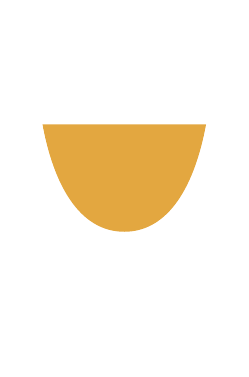
\begin{tikzpicture}[x=1cm,y=1cm,scale=1.05]
    \fill[Honey] (-0.99,1.60) .. controls (-0.83,0.75) and (-0.48,0.30) .. (0,0.30)
      .. controls (0.48,0.30) and (0.83,0.75) .. (0.99,1.60) -- cycle;
    \draw[white,line width=1.1pt] (-1.15,2.75) -- (-1.05,1.90)
      .. controls (-0.95,0.80) and (-0.50,0.25) .. (0,0.25)
      .. controls (0.50,0.25) and (0.95,0.80) .. (1.05,1.90) -- (1.15,2.75) -- cycle;
    \draw[white,line width=1.1pt] (0,0.25) -- (0,-1.1);
    \draw[white,line width=1.1pt] (-0.72,-1.1) -- (0.72,-1.1);
    \draw[white,opacity=0.65,line width=1.2pt] (-0.83,2.40) -- (-0.76,1.94);
  \end{tikzpicture}}
% Qvevri esquemático: vaso de argila em contato com o solo.
\newcommand{\qvevri}{%
  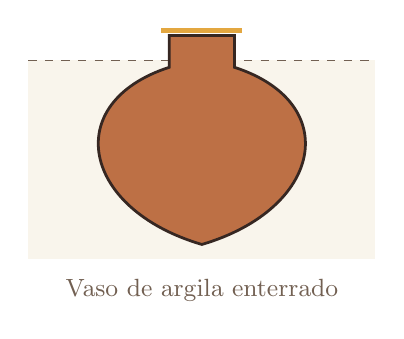
\begin{tikzpicture}[scale=0.90]
    \fill[Cream] (-2.45,-2.2) rectangle (2.45,0.6);
    \draw[Muted,dashed] (-2.45,0.6) -- (2.45,0.6);
    \fill[Amber!80] (-0.46,0.95) -- (-0.46,0.5)
      .. controls (-2.0,-0.0) and (-1.70,-1.50) .. (0,-2.0)
      .. controls (1.70,-1.50) and (2.0,-0.0) .. (0.46,0.5) -- (0.46,0.95) -- cycle;
    \draw[Ink,line width=1pt] (-0.46,0.95) -- (-0.46,0.5)
      .. controls (-2.0,-0.0) and (-1.70,-1.50) .. (0,-2.0)
      .. controls (1.70,-1.50) and (2.0,-0.0) .. (0.46,0.5) -- (0.46,0.95) -- cycle;
    \draw[Honey,line width=2pt] (-0.57,1.02) -- (0.57,1.02);
    \node[font=\small,text=Muted] at (0,-2.65) {Vaso de argila enterrado};
  \end{tikzpicture}}

\title{\Titulo}
\author{\Autor}
\hypersetup{pdftitle={Vinho laranja: das cascas à identidade sensorial},pdfauthor={\Autor}}

\begin{document}

% INTRODUÇÃO — apresenta o tema e a pergunta que guia a fala.
\section{Introdução}

% SLIDE 1 — ABERTURA | 0:25
% Fotografia à direita; textos em painel escuro para manter contraste.
\begin{frame}[plain]
  \begin{tikzpicture}[remember picture,overlay]
    \fill[Ink] (current page.south west) rectangle (current page.north east);
    \node[anchor=south west,inner sep=0pt] at ([xshift=9.2cm]current page.south west)
      {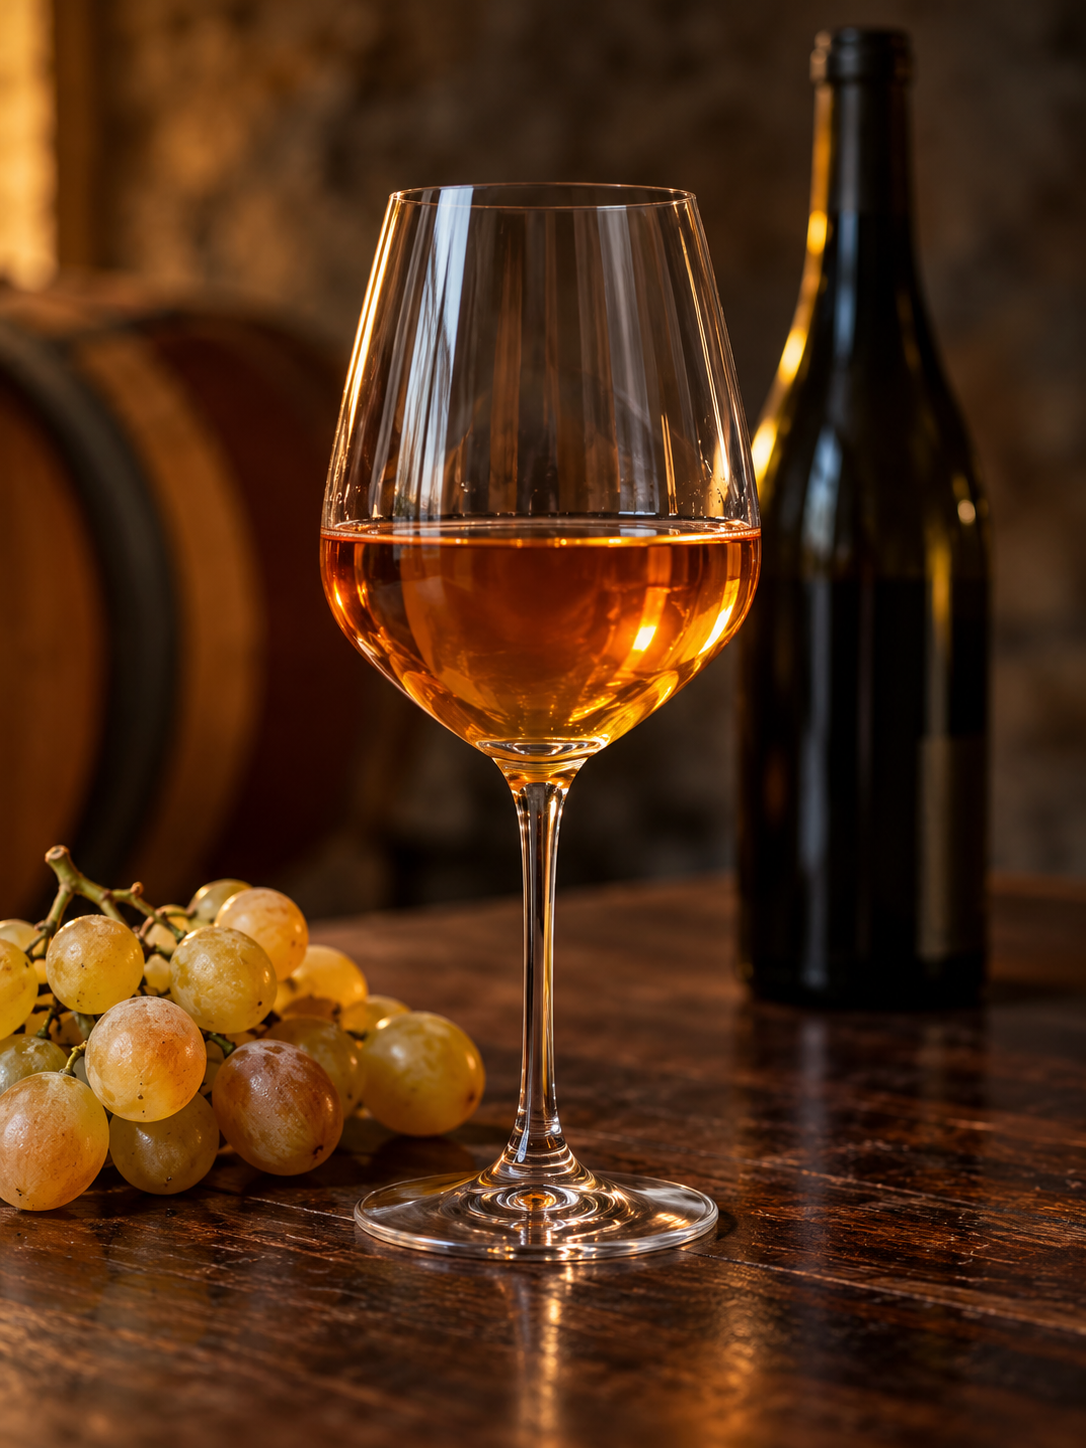
\includegraphics[width=6.8cm,height=9cm]{assets/hero.png}};
    \begin{scope}[shift={(current page.south west)},x=\paperwidth,y=\paperheight]
      \node[anchor=west,text=Honey,font=\small\bfseries] at (0.065,0.86) {CIÊNCIA E TECNOLOGIA DO VINHO};
      \node[anchor=west,text=white,align=left,font=\fontsize{34}{39}\selectfont\bfseries]
        at (0.065,0.57) {\TituloCapa};
      \node[anchor=west,text=Cream,align=left,text width=7.1cm,font=\large]
        at (0.065,0.30) {\Subtitulo};
      \draw[Honey,line width=1.2pt] (0.065,0.22) -- (0.20,0.22);
      \node[anchor=west,text=Cream,font=\small] at (0.065,0.14) {\Autor};
      \node[anchor=west,text=Honey,font=\fontsize{6.5}{8}\selectfont]
        at (0.065,0.055) {Fotos ilustrativas geradas por IA};
    \end{scope}
  \end{tikzpicture}
\end{frame}

% SLIDE 2 — INTRODUÇÃO HISTÓRICA | 0:40
\begin{frame}[t]{Introdução: raízes na antiga Geórgia}
  \framesubtitle{Da tradição georgiana ao vinho branco com maceração}
  \vspace{0.18cm}
  \begin{columns}[T,onlytextwidth]
    \begin{column}{0.46\textwidth}
      \kicker{GEÓRGIA \quad | \quad c. 6000--5800 a.C.}
      \bodytext{\textbf{Há cerca de 8 mil anos,} já se produzia vinho na região.}
      \vspace{0.16cm}
      \textrow{ONDE FICA?}{No Cáucaso, entre Europa e Ásia, junto ao mar Negro.}
      \textrow{RAÍZES DO VINHO LARANJA}{O estilo se liga à tradição georgiana
        de fermentar uvas brancas com as cascas.}
      \photocaption{A datação é de vinho em geral; não determina quando o estilo laranja foi inventado.}
    \end{column}
    \begin{column}{0.50\textwidth}
      % Não recortar: o globo e os rótulos fazem parte da imagem.
      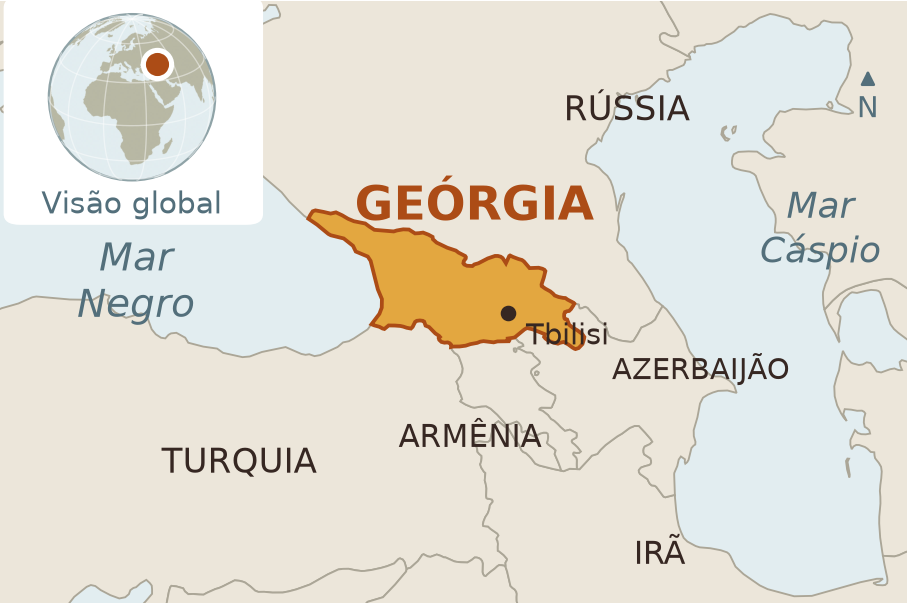
\includegraphics[width=\linewidth]{assets/mapa_georgia.png}
      \photocaption{Geórgia em âmbar. Base cartográfica: Natural Earth (domínio público).}
    \end{column}
  \end{columns}
  \source{[2], [4], [9]; localização: \href{https://georgia.travel/why-georgia-geography}{Georgia Travel}; mapa: \href{https://www.naturalearthdata.com/}{Natural Earth}}
\end{frame}

% DESENVOLVIMENTO — compara os estilos e explica o processo.
\section{Desenvolvimento}

% SLIDE 3 — COMPARAÇÃO COM OS VINHOS CONVENCIONAIS | 1:00
\begin{frame}[t]{Laranja, branco e tinto: qual é a diferença?}
  \framesubtitle{Comparação de estilos usuais de elaboração}
  \vspace{0.18cm}
  % Todas as células centralizadas na horizontal e na vertical, inclusive os critérios.
  % A configuração fica restrita a esta tabela.
  {\fontsize{11}{13.5}\selectfont
    \AlinharTabela
    \renewcommand{\arraystretch}{1.06}
    \setlength{\extrarowheight}{1pt}
    \setlength{\aboverulesep}{0pt}
    \setlength{\belowrulesep}{0pt}
    \setlength{\tabcolsep}{0.20cm}
    \arrayrulecolor{Honey!50}
    \begin{tabularx}{\textwidth}{>{\centering\arraybackslash\bfseries}m{2.60cm}
      >{\centering\arraybackslash}X
      >{\columncolor{Cream}\centering\arraybackslash}X
      >{\centering\arraybackslash}X}
      \rowcolor{Ink}
      \textcolor{white}{Critério} &
        \color{white}\textbf{Branco}\par convencional &
        \cellcolor{Amber}\color{white}\textbf{Vinho}\par\textbf{laranja} &
        \color{white}\textbf{Tinto}\par convencional \\
      \midrule
      Uvas & Em geral, brancas & \textcolor{Amber}{\textbf{Brancas}} & Tintas \\
      \midrule
      Cascas na fermentação & Em geral, sem cascas & \textcolor{Amber}{\textbf{Com cascas}} &
        Em geral, com cascas \\
      \midrule
      Cor usual & Palha a amarelo & Dourado a âmbar & Tons de vermelho \\
      \midrule
      Taninos e textura & Em geral, discretos &
        Podem ser mais perceptíveis & Variam com a uva e a extração \\
      \bottomrule
    \end{tabularx}\par
    \arrayrulecolor{black}}
  \callout{\centering\textbf{Ideia-chave:} uvas brancas com uma maceração semelhante à dos tintos.}
  \photocaption{Padrões usuais: uva, maceração e evolução alteram cor e textura. Há exceções, inclusive brancos feitos de uvas tintas.}
  \source{[1], [4], [7], [8]}
\end{frame}

% SLIDE 4 — FERMENTAÇÃO EM QVEVRI E TEMPOS | 1:10
\begin{frame}[t]{Como funciona a fermentação em qvevri?}
  \framesubtitle{Exemplo tradicional de Kakheti, na Geórgia, para uvas brancas}
  \vspace{0.16cm}
  \begin{columns}[T,onlytextwidth]
    \begin{column}{0.32\textwidth}
      \photo{assets/qvevri.png}{4.60cm}{3.00cm}
      \photocaption{Vasos de argila enterrados: cena ilustrativa por IA.}
      \vspace{0.14cm}
      \smalltext{\textbf{Total: 5--6 meses.}\\Inclui a alcoólica.}
      \photocaption{Tempos variáveis. Maturação adicional conforme o estilo.}
    \end{column}
    \begin{column}{0.64\textwidth}
      \textrow{01 \quad CARGA \quad | \quad NA VINDIMA}{Mosto, cascas e sementes entram no qvevri limpo.}
      \textrow{02 \quad FERMENTAÇÃO ALCOÓLICA \quad | \quad $\sim$20--40 DIAS}{Leveduras formam álcool e CO$_2$; as cascas flutuantes são submersas várias vezes ao dia.}
      \textrow{03 \quad VEDAÇÃO \quad | \quad APÓS AS FERMENTAÇÕES}{Os sólidos sedimentam. Após a malolática, veda-se o vaso; o contato com cascas continua.}
      \textrow{04 \quad TRASFEGA \quad | \quad $\sim$5--6 MESES DESDE O INÍCIO}{Na primavera georgiana, separar sólidos e trasfegar.}
    \end{column}
  \end{columns}
  \source{[2], National Wine Agency: método de Kakheti e tempos de elaboração}
\end{frame}

% SLIDE 5 — DA COLHEITA AO ENVASE | 1:40
% A figura apoia a explicação; o fluxograma continua sendo o elemento principal.
\begin{frame}[t]{Como o vinho laranja é produzido}
  \framesubtitle{Da colheita e seleção das uvas brancas ao vinho na garrafa}
  \vspace{0.10cm}
  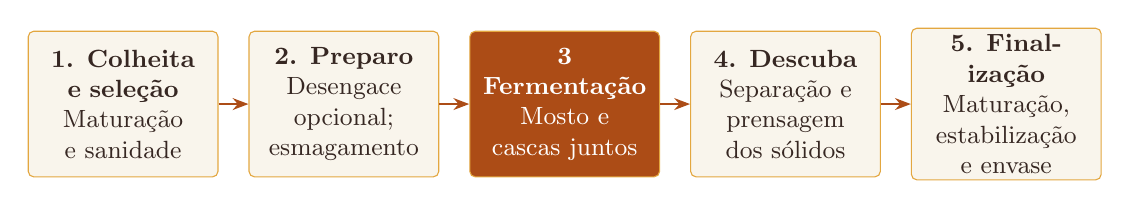
\begin{tikzpicture}[
    stagebox/.style={draw=Honey,fill=Cream,rounded corners=2pt,text=Ink,
      align=center,text width=2.25cm,minimum height=1.85cm,inner sep=0.08cm,
      font=\fontsize{9}{11}\selectfont},
    flow/.style={-{Stealth[length=2mm]},Amber,line width=0.9pt}]
    \node[stagebox] (a) {\textbf{1. Colheita}\\\textbf{e seleção}\\Maturação e sanidade};
    \node[stagebox,right=0.38cm of a] (b) {\textbf{2. Preparo}\\Desengace\\opcional;\\esmagamento};
    \node[stagebox,fill=Amber,text=white,right=0.38cm of b] (c) {\textbf{3}\\\textbf{Fermentação}\\Mosto e cascas juntos};
    \node[stagebox,right=0.38cm of c] (d) {\textbf{4. Descuba}\\Separação e prensagem dos sólidos};
    \node[stagebox,right=0.38cm of d] (e) {\textbf{5. Finalização}\\Maturação, estabilização e envase};
    \draw[flow] (a) -- (b); \draw[flow] (b) -- (c);
    \draw[flow] (c) -- (d); \draw[flow] (d) -- (e);
  \end{tikzpicture}
  \vspace{0.12cm}
  \begin{columns}[T,onlytextwidth]
    \begin{column}{0.32\textwidth}
      \photo{assets/maceracao.png}{4.60cm}{2.20cm}
      \photocaption{Categoria OIV: mínimo de 1 mês de contato com as cascas.}
    \end{column}
    \begin{column}{0.64\textwidth}
      \textrow{DO VINHEDO À RECEPÇÃO}{Colher pela maturação; transportar sem demora e retirar uvas deterioradas ou impurezas.}
      \textrow{FERMENTAÇÃO + MACERAÇÃO}{Leveduras geram etanol e CO$_2$; as cascas liberam cor, aromas e taninos. O contato pode seguir após a alcoólica.}
    \end{column}
  \end{columns}
  \source{[1], [3], [7]}
\end{frame}

% SLIDE 6 — ANATOMIA DA UVA | 1:10
\begin{frame}[t]{Cada parte da baga contribui de um jeito}
  \framesubtitle{O contato com cascas e sementes modifica o que passa para o mosto}
  \vspace{0.22cm}
  \begin{columns}[T,onlytextwidth]
    \begin{column}{0.36\textwidth}
      \photo{assets/uvas.png}{5.18cm}{3.85cm}
      \photocaption{Baga aberta: imagem ilustrativa, não um corte anatômico técnico.}
    \end{column}
    \begin{column}{0.60\textwidth}
      \textrow{CASCA \quad | \quad AROMAS E FENÓLICOS}{Contribui para a cor, os
        aromas e a estrutura. A composição varia com a cultivar.}
      \textrow{POLPA \quad | \quad MOSTO E FERMENTAÇÃO}{Principal fonte de líquido,
        açúcares fermentescíveis, acidez e nutrientes.}
      \textrow{SEMENTES \quad | \quad TANINOS E TEXTURA}{Contribuem para a estrutura;
        extração excessiva pode acentuar amargor e adstringência.}
    \end{column}
  \end{columns}
  \callout{\textbf{Na maturação:} açúcar, acidez, pH e fenólicos orientam a colheita e a extração.}
  \source{[3], [4], [7]}
\end{frame}

% SLIDE 7 — PERFIL SENSORIAL | 1:00
\begin{frame}[t]{O que pode aparecer na taça?}
  \framesubtitle{Uma família de estilos, com diferentes expressões sensoriais}
  \vspace{0.18cm}
  \photo{assets/tacas.png}{14.4cm}{1.85cm}
  \vspace{0.15cm}
  \begin{columns}[T,onlytextwidth]
    \begin{column}{0.315\textwidth}
      \sensory{VISUAL}{Dourado a âmbar}{Intensidade ligada à uva, à maceração e à evolução do vinho.}
    \end{column}
    \begin{column}{0.315\textwidth}
      \sensory{AROMAS}{Diversidade}{Frutas secas, casca cítrica e nozes podem aparecer, conforme o estilo.}
    \end{column}
    \begin{column}{0.315\textwidth}
      \sensory{BOCA}{Textura}{Pode haver mais estrutura e adstringência do que em brancos convencionais.}
    \end{column}
  \end{columns}
  \vspace{0.13cm}
  {\fontsize{9.5}{12}\selectfont
    \textbf{Cor não determina doçura:} o açúcar residual depende da condução da fermentação.\par
    \textbf{Diversidade tecnológica:} o estilo não exige ânfora nem ausência de aditivos.\par}
  \source{[4], [5], [6]}
\end{frame}

% SLIDE 8 — CONTROLE DE PROCESSO | 1:05
\begin{frame}[t]{Como equilibrar extração e qualidade?}
  \framesubtitle{As escolhas de processo precisam acompanhar o perfil desejado}
  \vspace{0.19cm}
  \begin{columns}[T,onlytextwidth]
    \begin{column}{0.63\textwidth}
      \textrow{01 \quad UVA E EXTRAÇÃO}{Cultivar, maturação e tempo orientam a extração; sementes verdes podem acentuar a adstringência.}
      \textrow{02 \quad FERMENTAÇÃO}{Acompanhar temperatura, açúcar, pH e acidez.}
      \textrow{03 \quad OXIGÊNIO E PROTEÇÃO}{Manejar oxigênio e SO$_2$ para limitar
        oxidação e alterações microbianas.}
      \textrow{04 \quad HIGIENE E ACOMPANHAMENTO}{Avaliar o vinho e controlar
        alterações microbianas durante o contato com os sólidos.}
    \end{column}
    \begin{column}{0.33\textwidth}
      \photo{assets/controle.png}{4.75cm}{4.10cm}
      \vspace{0.10cm}
      {\fontsize{10}{13}\selectfont\bfseries Mais extração não garante mais qualidade.
      O objetivo é o equilíbrio.\par}
    \end{column}
  \end{columns}
  \source{[4], [7]}
\end{frame}

% CONCLUSÃO — retoma o objetivo e fecha a mensagem central.
\section{Conclusão}

% SLIDE 9 — COMO O PROCESSO CONSTRÓI A IDENTIDADE | 0:50
\begin{frame}[plain]
  \begin{tikzpicture}[remember picture,overlay]
    \fill[Ink] (current page.south west) rectangle (current page.north east);
    \node[anchor=south west,inner sep=0pt] at ([xshift=9.2cm]current page.south west)
      {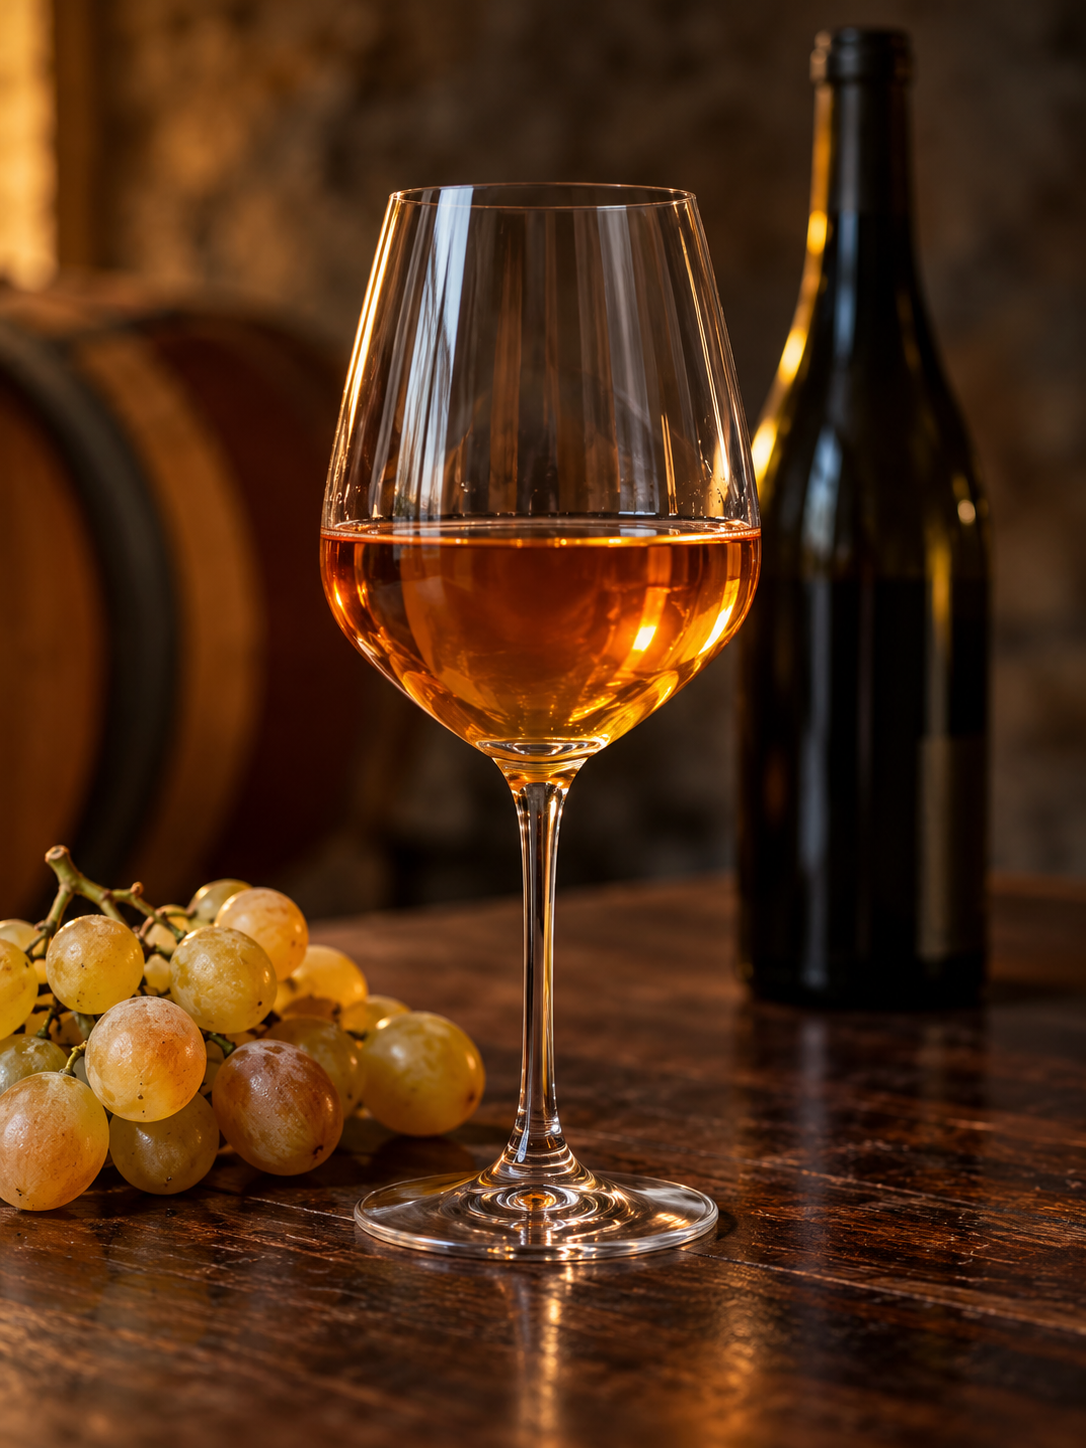
\includegraphics[width=6.8cm,height=9cm]{assets/hero.png}};
    \begin{scope}[shift={(current page.south west)},x=\paperwidth,y=\paperheight]
      \node[anchor=north west,text=Honey,font=\fontsize{9}{11}\selectfont\bfseries]
        at (0.065,0.92) {CONCLUSÃO \enspace\textbullet\enspace DO PROCESSO À TAÇA};
      \node[anchor=north west,text=white,text width=7.1cm,align=left,font=\fontsize{20}{24}\selectfont\bfseries]
        at (0.065,0.85) {Identidade construída\\pelo processo.};
      \node[anchor=north west,text=Honey,font=\fontsize{9}{11}\selectfont\bfseries]
        at (0.065,0.62) {CASCAS + TEMPO DE CONTATO};
      \node[anchor=north west,text=Cream,text width=7.1cm,align=left,font=\fontsize{11.5}{14.5}\selectfont]
        at (0.065,0.57) {Mais extração pode ampliar cor, taninos e adstringência.};
      \node[anchor=north west,text=Honey,font=\fontsize{9}{11}\selectfont\bfseries]
        at (0.065,0.44) {FERMENTAÇÃO};
      \node[anchor=north west,text=Cream,text width=7.1cm,align=left,font=\fontsize{11.5}{14.5}\selectfont]
        at (0.065,0.39) {A condução muda aromas, álcool e açúcar residual.};
      \node[anchor=north west,text=Honey,font=\fontsize{9}{11}\selectfont\bfseries]
        at (0.065,0.26) {MATURAÇÃO + PROTEÇÃO};
      \node[anchor=north west,text=Cream,text width=7.1cm,align=left,font=\fontsize{11.5}{14.5}\selectfont]
        at (0.065,0.21) {Recipiente e oxigênio mudam aromas e estabilidade.};
      \node[anchor=west,text=Honey,font=\fontsize{6.5}{8}\selectfont]
        at (0.065,0.035) {Fontes: [1], [4], [5].\quad Imagem ilustrativa por IA};
    \end{scope}
  \end{tikzpicture}
\end{frame}

\section{Referências}

% SLIDE 10 — FONTES | 0:20
% Os links são clicáveis no PDF. As notas completas estão em roteiro.md.
\begin{frame}[t]{Fontes e leitura complementar}
  \framesubtitle{Material de aula, normas e referências técnicas}
  \vspace{0.12cm}
  \fontsize{9}{11}\selectfont
  \begin{enumerate}
    \setlength{\itemsep}{0.06cm}
    \item OIV. \textit{White wine with maceration}. Resolução OIV-ECO 647-2020.
      \href{https://www.oiv.int/public/medias/7584/oiv-eco-647-2020-en.pdf}{Definição e prescrições.}
    \item National Wine Agency, Geórgia. \textit{Qvevri Wine}.
      \href{https://wine.gov.ge/En/KvevriWine}{Tradição};
      \href{https://www.georgianwine.jp/wine-making/}{método de Kakheti e tempos de elaboração.}
    \item OIV. \textit{Maceration (General sheet)}. Resolução OIV/OENO 196/2009.
      \href{https://www.oiv.int/index.php/node/3466}{Definição e objetivo da maceração.}
    \item AWRI. \textit{Winemaking treatment -- Amber wine}.
      \href{https://www.awri.com.au/industry_support/winemaking_resources/winemaking-practices/winemaking-treatment-amber-wine/}{Processo, estilo e cuidados de elaboração.}
    \item Philipp, C. et al. \textit{The Influence of Prefermentation Skin Contact,
      Stabulation, and Skin Fermentation\ldots} Australian Journal of Grape and Wine Research, 2024.
      \href{https://doi.org/10.1155/2024/9843225}{DOI: 10.1155/2024/9843225.}
    \item WSET. \textit{What is orange wine? Understanding skin-contact white wines}. 2026.
      \href{https://www.wsetglobal.com/knowledge-centre/blog/2026/what-is-orange-wine-understanding-skin-contact-white-wines}{Estilos, tradição e características sensoriais.}
    \item Materiais de aula: aulas 6--8 (vinho tinto) e 10 (vinho branco), 2026.
      Aula 9 (cerveja): apenas princípios gerais de controle fermentativo, sem transpor etapas cervejeiras.
    \item WSET. \href{https://www.wsetglobal.com/knowledge-centre/blog/2021/september/23/what-determines-the-colour-of-wine}{\textit{What determines the colour of wine?}} 2021. Estilos e contato com cascas.
    \item McGovern, P. et al. \textit{Early Neolithic wine of Georgia in the South Caucasus}.
      PNAS, 2017. \href{https://doi.org/10.1073/pnas.1714728114}{DOI: 10.1073/pnas.1714728114.}
  \end{enumerate}
\end{frame}

\end{document}
